\documentclass[12pt, french]{article}

\usepackage{fancyhdr, fancybox, lastpage}
\usepackage[most]{tcolorbox}
\usepackage[a4paper, margin={0.3in, .75in}]{geometry}
\usepackage{wrapfig}
\pagestyle{fancy}
\renewcommand\headrulewidth{1pt}
\renewcommand\footrulewidth{1pt}
\fancyhf{}
\rhead{ \em{Zakaria Haouzan}}
\lhead[C]{\em{2ème année baccalauréat Sciences Mathématiques}}
\chead[C]{}
\rfoot[C]{}
\lfoot[R]{\emph{Propagation d’une onde lumineuse}}
\cfoot[]{\em{Page \thepage / \pageref{LastPage}}}


\newtcolorbox{Box2}[2][]{
                lower separated=false,
                colback=white,
colframe=white!20!black,fonttitle=\bfseries,
colbacktitle=white!30!gray,
coltitle=black,
enhanced,
attach boxed title to top left={yshift=-0.1in,xshift=0.15in},
title=#2,#1}


\begin{document}
\begin{center}

	\shadowbox { \vspace{-1cm}\bf{Propagation d’une onde lumineuse}}
\end{center}

\vspace{-0.4cm}
%%_________________________Exercice ! :"_________________________Exercice
   \begin{Box2}{Exercice 1 :  Choisir les bonnes réponses parmi celles qui sont proposées (QCM) : }
	   \begin{enumerate}
		   \item  le spectre de la lumière visible est formé de radiations dont les longueurs d’onde dans le vide sont
comprises entre :

(a)400mm et 800 mm \hspace{1cm}(b) 400$\mu$ et 800 $\mu m$ \hspace{1cm}(c) 400nm et 800 nm

\item la longueur d’onde $\lambda$ dans le vide d’une radiation de fréquence $\nu$ est donnée par la relation : 

	(a) $\lambda=c.\nu$ \hspace{3cm}(b) $\lambda=\frac{c}{\nu}$ \hspace{2.6cm}  (c) $\lambda=\frac{\nu}{c}$

\item le phénomène de diffraction permet de mettre en évidence :

	(a)le caractère ondulatoire de la lumière \hspace{0.5cm} (b) l’influence du milieu sur la vitesse de propagation

\item lors d’une expérience de diffraction d’un faisceau lumineux de longueur d’onde $\lambda$ par une fente de largeur a située à la distance D de l’écran, la largeur de la tache centrale observée sur l’écran est :

	(a) proportionnelle à a \hspace{0.6cm} (b) inversement proportionnelle à a \hspace{0.6cm} (c) indépendante de a

	(d) proportionnelle à $\lambda$ \hspace{0.6cm} (e) inversement proportionnelle à $\lambda$ \hspace{0.6cm} (f) indépendante de $\lambda$
	
	(g) proportionnelle à $D$ \hspace{0.6cm} (h) inversement proportionnelle à $D$ \hspace{0.6cm} (i) indépendante de $D$

\end{enumerate}
   \end{Box2}
   


%%_________________________Exercice !2 :"_________________________Exercice
\begin{Box2}{Exercice 2 :lampe à iode  }
%\begin{wrapfigure}{r}{0.26\textwidth}
  %\begin{center}
	  %\vspace{-1cm}
	%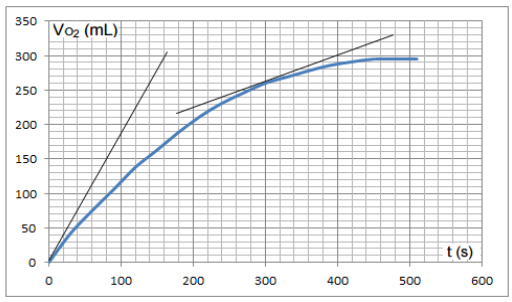
\includegraphics[width=0.24\textwidth]{./img/ex2.png}
  %\end{center}
%\end{wrapfigure}

Une lampe à iode émet de nombreuses radiations, les longueurs d’onde dans le vide de trois de ces
radiations sont : 512 nm, 534 nm et 563 nm.
\begin{enumerate}
	\item  Cette lampe émet-elle une lumière monochromatique ou polychromatique ?
	\item  Calculer la fréquence de ces radiations.
		Donnée : célérité de la lumière dans le vide $c=3.10^8 m/s$
\end{enumerate}

\end{Box2}

%%_________________________Exercice ! 3:"_________________________Exercice
\begin{Box2}{Exercice 3 : laser Y.A.G (Yttrium Alumimium Garnet)}

Un laser Y.A.G (Yttrium Alumimium Garnet) utilisé en médecine possède, dans le vide, une longueur
d’onde $\lambda_0 = 1060 nm$
\begin{enumerate}
\item Cette onde lumineuse est-elle visible ? dans quel domaine du spectre se situe-t-elle ?
\item  Calculer sa fréquence.
\item  Calculer la longueur d’onde $\lambda_1$ de ce laser dans un verre flint d’indice n = 1,58
\item Dans un verre crown, la longueur d’onde de ce laser est $\lambda_2 =716 nm$. Calculer l’indice de ce verre.
\end{enumerate}
\end{Box2}

%%_________________________Exercice 4 : _________________________Exercice
\begin{Box2}{Exercice 4 :onde monochromatique }

\begin{wrapfigure}{r}{0.28\textwidth}
  \begin{center}
	  \vspace{-0.8cm}
	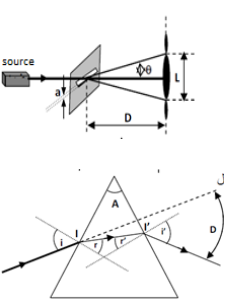
\includegraphics[width=0.28\textwidth]{./img/ex4.png}
  \end{center}
\end{wrapfigure}

Un laser émet une onde monochromatique de longueur d’onde $\lambda$, par
une ouverture de largeur $a$=$120\mu m$, il produit une tache lumineuse de
longueur L sur un écran situé à la distance $D = 1,5m$ de l’ouverture.

\textbf{1. }Donner le nom de ce phénomène.

\textbf{2. }démontrer la relation entre $a$, $L$, $D$ et $\theta$

\textbf{3. }Calculer la longueur d’onde pour $L= 1,6cm$
On attaque un prisme par le même faisceau lumineux.
Donnée : A=60°, i = 45°, n= 1,66 indice de réfraction du prisme

\textbf{4. }Définir une onde monochromatique.

\textbf{5. }Donner les lois de Descartes au point I et I’ on donne $n_{air} =1$

\textbf{6. }Rappeler les relations du prisme.

\textbf{7. }Donner les valeurs de r, r’, i, D

\textbf{8. }En remplace le laser par une source de lumière blanche .Quel phénomène sera-t-il mis en évidence ?

\end{Box2}
\begin{center}
   \Large{ \em{Exercices Supplémentaires}}
\end{center}




\begin{Box2}{Exercice 5 :longueur d’onde d’une lumière
monochromatique }
\begin{wrapfigure}{r}{0.4\textwidth}
  \begin{center}
	  \vspace{-0.6cm}
	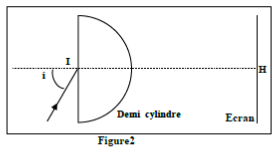
\includegraphics[width=0.4\textwidth]{./img/ex_5.png}
  \end{center}
\end{wrapfigure}

Un rayon lumineux $(R_1)$ monochromatique de fréquence $\nu_1 = 3,80.10^{14}$ Hz arrive sur la face plane d’un
demi-cylindre en verre transparent au point d’incidence I sous un angle d’incidence $i$=60°. 

Le rayon $(R_1)$ se réfracte au point I et arrive à l’écran vertical au point A (figure2).
On fait maintenant arriver un rayon lumineux monochromatique $(R_2)$ de fréquence $\nu_2$=$7,50.10^{14} Hz$
sur la face plane du demi-cylindre sous le même angle d’incidence i = 60°. 

On constate que le rayon $(R_2)$ se réfracte aussi au point I mais il arrive à l’écran vertical en un autre point B de tel sorte que
l’angle entre les deux rayons réfractés est $\alpha$=0,563°.

\underline{\textbf{Données :}}

\begin{itemize}
		\item L’indice de réfraction du verre pour le rayon lumineux de fréquence $\nu_1$ est $n_1$ = 1,626.
		\item  L’indice de réfraction de l’air est 1,00.
		\item  $c$=$3,00.10^8 m/s$.
\end{itemize}

\begin{enumerate}
	\item Montrer que la valeur de l’indice de réfraction du verre pour le rayon lumineux de fréquence $\nu_2$ est $n_2$=1,652.
	\item Trouver l’expression de la longueur d’onde $\lambda_2$ du rayon lumineux de fréquence $\nu_2$ dans le
verre, en fonction de $c$, $n_2$ et $\nu_2$. Calculer $\lambda_2$.
\end{enumerate}
\end{Box2}
%\vspace{2cm}
%\vspace{-0.7cm}
%%_________________________Exercice 5 : _________________________Exercice
%\begin{Box2}{Exercice 6 :Propagation d’une onde mécanique à la surface de l’eau  }
%4
%\end{Box2}
%%_________________________Exercice 6 : _________________________Exercice
%\begin{Box2}{Exercice 6 : échographie}
%%\begin{wrapfigure}{r}{0.2\textwidth}
  %%\begin{center}
	  %%\vspace{-0.6cm}
	%%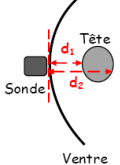
\includegraphics[width=0.2\textwidth]{./img/Exercice6.png}
  %%\end{center}
%%\end{wrapfigure}
%6
%\end{Box2}

\end{document}
